%\documentclass{beamer} 
\documentclass[handout]{beamer} % sin pausas
\usetheme{CambridgeUS}

\usepackage[utf8]{inputenc}%esto permite (en Windows) escribir directamente 
\usepackage{graphicx}
\usepackage{array}
\usepackage{tikz} 
\usetikzlibrary{shapes,arrows,babel,decorations.pathreplacing}
\usepackage{verbatim} 
\usepackage{xcolor} 
\usepackage{amsgen,amsmath,amstext,amsbsy,amsopn,amsfonts,amssymb}
\usepackage{amsthm}
\usepackage{tikz}
\usepackage{tkz-graph}
\usepackage{mathtools}
\usepackage{xcolor}

%\setbeamertemplate{background}[grid][step=8 ]
\setbeamertemplate{itemize item}{$\circ$}
\setbeamertemplate{enumerate items}[default]

\definecolor{links}{HTML}{2A1B81}
\hypersetup{colorlinks,linkcolor=,urlcolor=links}

\newcommand{\img}{\operatorname{Im}}
\newcommand{\nuc}{\operatorname{Nu}}
\newcommand\im{\operatorname{Im}}
\renewcommand\nu{\operatorname{Nu}}
\newcommand{\la}{\langle}
\newcommand{\ra}{\rangle}
\renewcommand{\t}{{\operatorname{t}}}
\renewcommand{\sin}{{\,\operatorname{sen}}}
\newcommand{\Q}{\mathbb Q}
\newcommand{\R}{\mathbb R}
\newcommand{\C}{\mathbb C}
\newcommand{\K}{\mathbb K}
\newcommand{\F}{\mathbb F}
\newcommand{\Z}{\mathbb Z}

\renewcommand{\figurename }{Figura}
%\usepackage{enumitem}
%\setlist[itemize]{itemsep=10pt, label={$\circ$}}
%\newtheorem{teorema}{Teorema}
%\newtheorem{corolario}[teorema]{Corolario}
%\newtheorem{proposicion}[teorema]{Proposición}

%\theoremstyle{definition}
%\newtheorem{definicion}[theorem]{Definici\'on}
%\newtheorem{ejemplo}[theorem]{Ejemplo}
%\newtheorem{pregunta}[equation]{Pregunta}
%\newtheorem{step}{Paso}

\setbeamercolor{block}{fg=red, bg=red!40!white}
\setbeamercolor{block example}{use=structure,fg=black,bg=white!20!white}

\renewenvironment{block}[1]% environment name
{% begin code
	\par\vskip .2cm%
	{\color{blue}#1}%
	\vskip .2cm
}%
{%
	\vskip .2cm}% end code


\renewenvironment{alertblock}[1]% environment name
{% begin code
	\par\vskip .2cm%
	{\color{red!80!black}#1}%
	\vskip .2cm
}%
{%
	\vskip .2cm}% end code


\renewenvironment{exampleblock}[1]% environment name
{% begin code
	\par\vskip .2cm%
	{\color{blue}#1}%
	\vskip .2cm
}%
{%
	\vskip .2cm}% end code

\newenvironment{exercise}[1]% environment name
{% begin code
	\par\vspace{\baselineskip}\noindent
	\textbf{Ejercicio (#1)}\begin{itshape}%
		\par\vspace{\baselineskip}\noindent\ignorespaces
	}%
	{% end code
	\end{itshape}\ignorespacesafterend
}


\newenvironment{definicion}% environment name
{% begin code
	\par\vskip .2cm%
	{\color{blue}Definición}%
	\vskip .2cm
}%
{%
	\vskip .2cm}% end code

\newenvironment{observacion}% environment name
{% begin code
	\par\vskip .2cm%
	{\color{blue}Observación}%
	\vskip .2cm
}%
{%
	\vskip .2cm}% end code

\newenvironment{ejemplo}% environment name
{% begin code
	\par\vskip .2cm%
	{\color{blue}Ejemplo}%
	\vskip .2cm
}%
{%
	\vskip .2cm}% end code

\newenvironment{ejercicio}% environment name
{% begin code
	\par\vskip .2cm%
	{\color{blue}Ejercicio}%
	\vskip .2cm
}%
{%
	\vskip .2cm}% end code


\renewenvironment{proof}% environment name
{% begin code
	\par\vskip .2cm%
	{\color{blue}Demostración}%
	\vskip .2cm
}%
{%
	\vskip .2cm}% end code



\newenvironment{demostracion}% environment name
{% begin code
	\par\vskip .2cm%
	{\color{blue}Demostración}%
	\vskip .2cm
}%
{%
	\vskip .2cm}% end code

\newenvironment{idea}% environment name
{% begin code
	\par\vskip .2cm%
	{\color{blue}Idea de la demostración}%
	\vskip .2cm
}%
{%
	\vskip .2cm}% end code

\newenvironment{solucion}% environment name
{% begin code
	\par\vskip .2cm%
	{\color{blue}Solución}%
	\vskip .2cm
}%
{%
	\vskip .2cm}% end code



\newenvironment{lema}% environment name
{% begin code
	\par\vskip .2cm%
	{\color{blue}Lema}\begin{itshape}%
		\par\vskip .2cm
	}%
	{% end code
	\end{itshape}\vskip .2cm\ignorespacesafterend
}

\newenvironment{proposicion}% environment name
{% begin code
	\par\vskip .2cm%
	{\color{blue}Proposición}\begin{itshape}%
		\par\vskip .2cm
	}%
	{% end code
	\end{itshape}\vskip .2cm\ignorespacesafterend
}

\newenvironment{teorema}% environment name
{% begin code
	\par\vskip .2cm%
	{\color{blue}Teorema}\begin{itshape}%
		\par\vskip .2cm
	}%
	{% end code
	\end{itshape}\vskip .2cm\ignorespacesafterend
}


\newenvironment{corolario}% environment name
{% begin code
	\par\vskip .2cm%
	{\color{blue}Corolario}\begin{itshape}%
		\par\vskip .2cm
	}%
	{% end code
	\end{itshape}\vskip .2cm\ignorespacesafterend
}

\newenvironment{propiedad}% environment name
{% begin code
	\par\vskip .2cm%
	{\color{blue}Propiedad}\begin{itshape}%
		\par\vskip .2cm
	}%
	{% end code
	\end{itshape}\vskip .2cm\ignorespacesafterend
}

\newenvironment{conclusion}% environment name
{% begin code
	\par\vskip .2cm%
	{\color{blue}Conclusión}\begin{itshape}%
		\par\vskip .2cm
	}%
	{% end code
	\end{itshape}\vskip .2cm\ignorespacesafterend
}




\title[Clase 5 - Rectas y planos 3]{Álgebra/Álgebra II \\ Clase 5 - Rectas y planos 3}
%\author[C. Olmos / A. Tiraboschi]{Carlos Olmos / Alejandro Tiraboschi}
\institute[]{\normalsize FAMAF / UNC
	\\[\baselineskip] ${}^{}$
	\\[\baselineskip]
}
\date[08/09/2020]{8 de septiembre de 2020}




\begin{document}
	
	\frame{\titlepage} 
	

\begin{frame}
	
	En estas transparencias revisaremos los conceptos
	\begin{itemize}
		\item ecuación implícita de la recta o la recta perpendicular a una direcci\'on dada,
		\item la recta que pasa por dos puntos dados,
		\item ecuación paramétrica de la recta
		\item el plano en $\R^3$ perpendicular a un vector dado, 
		\item ecuación paramétrica del plano.
	\end{itemize}
	
	
	Veremos ejemplos prácticos de como pasas de la ecuación implícita de la recta y el plano a la ecuación paramétrica y viceversa. 
	
\end{frame}


\begin{frame}\frametitle{Definición implícita de la recta en $\R^2$}
	\begin{definicion} Una  \textit{recta}\index{recta} está formada por el conjunto de puntos $(x,y)$ en $\R^2$ que satisfacen la ecuación
		\begin{equation}\label{eq-implicita-de-la-recta}
		ax +by =c,
		\end{equation}
		con $a,b,c \in \R$ y tal que $a,b$ no pueden ser simultáneamente $0$. 
		\pause
		\vskip .3cm
		Más formalmente, la recta es el conjunto
		\begin{equation*}
		L = \{ (x,y) \in \R^2:ax +by =c\}.
		\end{equation*}
	\end{definicion}
	
	\pause
	\begin{observacion}
		\begin{itemize}
			\item Si $b\ne0$, entonces la recta es \, $y= -\displaystyle\frac{a}{b}x + \displaystyle\frac{c}{b}$, 
			\item si $b=0$,  entonces $a\ne 0$ y la recta es \, $x =\displaystyle\frac{c}{a}$.
		\end{itemize}
	\end{observacion}
	
\end{frame}




\begin{frame}
	\begin{observacion}
		\textit{La ecuación implícita de la recta $L$ perpendicular a $(a,b)$ y que pasa por $p = (x_0,y_0)$ es
			\begin{equation*}
			ax +by = \langle (x_0,y_0), (a,b) \rangle.
			\end{equation*}}
	\end{observacion}

		\begin{center}
		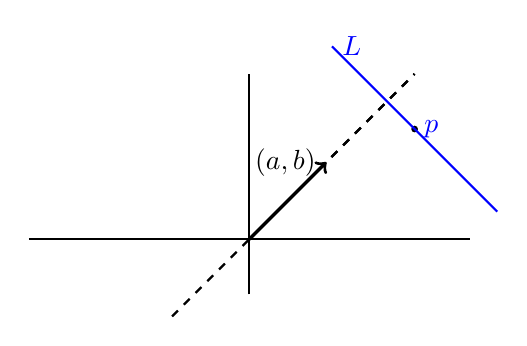
\begin{tikzpicture}[scale=0.7]
		\def\vx{3}
		\def\vy{2}
		\def\wx{4}
		\def\wy{1}	
		\def\tv{3.0}
		\def\tw{1.4}
		\def\taa{1.5}
		\def\tab{-1.5}
		\def\rr{\tv*\vy-\tv*\wy}	
		\def\ss{\tv*\wx-\tv*\vx}		
		\def\rrm{-\tw*\vy+\tw*\wy}	
		\def\ssm{-\tw*\wx+\tw*\vx}		
		\draw[thick,-] (-4,0) -- (4,0);
		\draw[thick,-] (0,-1) -- (0,3);
		%\node[inner sep=1.5pt,fill,circle] at (\vx,\vy) {};
		\draw[fill] (\vx,\vy) circle [radius=0.05];
		\node[blue,right] at (\vx,\vy) {$p$};
		% 		\draw[very thick,->] (0,0) -- (\wx,\wy) node[above]{\;$v$};
		% 		\draw[very thick,->] (0,0) -- (\wx-\vx,\wy-\vy) node[right]{$v-v_0$};
		\draw[thick,blue,-] (\vx- \tab*\vx + \tab*\wx ,\vy - \tab*\vy + \tab*\wy) node[right] {$L$} --  (\vx- \taa*\vx + \taa*\wx ,\vy - \taa*\vy + \taa*\wy);
		\draw[very thick,->] (0,0) -- (\tw*\vy-\tw*\wy,\tw*\wx-\tw*\vx) node[left]{$(a,b)$};
		\draw[dashed, thick,-] (0,0) -- (\rr,\ss);
		\draw[dashed, thick,-] (0,0) -- (\rr,\ss);
		\draw[dashed, thick,-] (\rrm,\ssm) -- (0,0);
		%\draw[dashed,thick] (0,0) (\tw*\wx,\tw*\wy) -- (\vx+\tw*\wx,\vy+\tw*\wy+0.1);
		%\node[inner sep=1.5pt,fill,circle,blue] at (\vx+\tw*\wx+0.04*\wx,\vy+\tw*\wy+0.04*\wy)  {};
		%\node[right] at (\vx+\tw*\wx,\vy+\tw*\wy+0.1){$v+tw$};
		\end{tikzpicture}
	\end{center} 
	\vskip 0.5cm
	Ver en GeoGebra: \href{https://www.geogebra.org/m/uu4gzhfr}{\beamergotobutton{https://www.geogebra.org/m/uu4gzhfr}}
\end{frame}


	
\begin{frame}{Definición paramétrica de la recta}
	
	
	\begin{definicion}
		Sean $v, w \in \R^2$ tal que  $w \not=0$. Sea 
		\begin{equation*}
		L = \{v + tw: t \in \R\}. 
		\end{equation*}
		Diremos entonces que  \textit{$L$ es la recta que pasa por $v$ paralela a $w$.} 
	\end{definicion}
	\vskip .3cm	\pause 
	Observemos que la recta $L$ está dada por todos los puntos que se obtienen de la función
	\begin{equation}\label{eq-ecuacion-parametrica-recta}
	X(t) =v +tw, \quad \text{para $t \in \R$.} 
	\end{equation} 
	\vskip .3cm	\pause 
	En  el espacio $\R^2$, diremos que (\ref{eq-ecuacion-parametrica-recta}) es la \textit{ecuación paramétrica} o la \textit{representación paramétrica}\index{recta!ecuación paramétrica} de la recta $L$ que pasa por el punto $v$ y es paralela a $w \ne 0$.
	
\end{frame}



\begin{frame}
	Podemos representar una recta dada en forma paramétrica:
	\vskip 0.8cm
	\begin{center}
		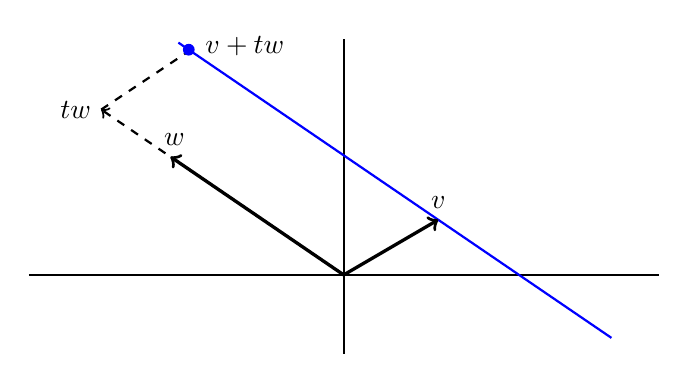
\begin{tikzpicture}
		\def\vx{1.2}
		\def\vy{0.7}
		\def\wx{-2.2}
		\def\wy{1.5}	
		\def\tw{1.4}					
		\draw[thick,-] (-4,0) -- (4,0);
		\draw[thick,-] (0,-1) -- (0,3);
		\draw[thick,blue,-] (\vx+1.5*\wx,\vy+1.5*\wy) -- (\vx-1*\wx,\vy-1*\wy);
		%\node[inner sep=1.5pt,fill,circle] at (\vx,\vy) {};
		\draw[very thick,->] (0,0) -- (\vx,\vy) node[above]{$v$};
		\draw[very thick,->] (0,0) -- (\wx,\wy) node[above]{\;$w$};
		\draw[dashed, thick,->] (0,0) -- (\tw*\wx,\tw*\wy) node[left]{$tw$};
		\draw[dashed,thick] (0,0) (\tw*\wx,\tw*\wy) -- (\vx+\tw*\wx,\vy+\tw*\wy+0.1);
		\node[inner sep=1.5pt,fill,circle,blue] at (\vx+\tw*\wx+0.04*\wx,\vy+\tw*\wy+0.04*\wy)  {};
		\node[right] at (\vx+\tw*\wx,\vy+\tw*\wy+0.1){$v+tw$};
		\end{tikzpicture}
	\end{center} 
\vskip 0.5cm
Ver en GeoGebra: \href{https://www.geogebra.org/m/memspwaa}{\beamergotobutton{https://www.geogebra.org/m/memspwaa}}
\end{frame}

\begin{frame}{De ecuación ecuación implícita a paramétrica}
	\begin{ejemplo}
	
			Encontrar la ecuación paramétrica de la recta 
			\begin{equation*}\label{eq-impl-rec-ej}
			5x + y = 11,
			\end{equation*}
	\end{ejemplo}
	\begin{solucion}\pause
	
			Observar  que $y = -5x +11$, luego la recta es
			\begin{align*} 
				L&=\{(x,y): y = -5x + 11, x \in \R \} \\
				&= \{(x, -5x + 11): x \in \R \} \\
				&= \{(t, -5t + 11): t \in \R \}\\
				&= \{(0,11) + t(-1, -5): t \in \R \}
			\end{align*}
			
			
				\qed  
	\end{solucion}	
	
	
\end{frame}


\begin{frame}{De ecuación paramétrica a ecuación implícita}
	\begin{ejemplo}
		{\footnotesize
		Encontrar la representación implícita de la recta 
		\begin{equation*}
		X(t)= (2,1)+ t(-1,5) = (2-t,1+5t).
		\end{equation*}\pause}
	\end{ejemplo}\vskip -.4cm
	\begin{solucion}\pause
		{\footnotesize
			Coordenada a coordenada:  
			\begin{equation}\label{eq-par-des-ej}
			x = 2 - t, \qquad\quad y = 1 + 5t. \qquad\quad\tag{*}
			\end{equation}
			
			
			
			Despejando $t$ de la primera ecuación obtenemos $t = 2-x$. 
			
			\vskip .3cm \pause
			
			Reemplazando este valor de $t$  en la segunda ecuación obtenemos
			\begin{equation*}
			y = 1 + 5t=1 + 5(2-x) = 11- 5x,
			\end{equation*}\pause
			luego
			\begin{equation}\label{eq-impl-rec-ej}
			5x + y = 11,\tag{**}
			\end{equation}
			que es la ecuación implícita de la recta.	\qed  }
	\end{solucion}	
	
	
\end{frame}

\begin{frame}{Recta que pasa por un punto perpendicular a un vector}
	\begin{ejemplo}{Pregunta (Ejericicio 13,14)}
	Sean $(a,b),(x_0,y_0)\in\R^2$. 
	
	\
	
	¿Cu\'al es la forma param\'etrica de la recta $L$ perpendicular a $(a,b)$ y que pasa por $p=(x_0,y_0)$?
	
\end{ejemplo}

\begin{solucion}
	Para responder a la pregunta, comencemos por recordar que dos vectores en $\R^2$ son perpendiculares si el producto escalar entre ellos es nulo.
	
	\
	
	Elijamos $w\in\R^2$ no nulo tal que $\langle w,(a,b)\rangle=0$. (¿Existe?)
	
	\
	
	Entonces la recta que buscamos es la recta que pasa por $p$ con direcci\'on $w$.
	

\end{solucion}
\end{frame}



\begin{frame}
		\begin{center}
		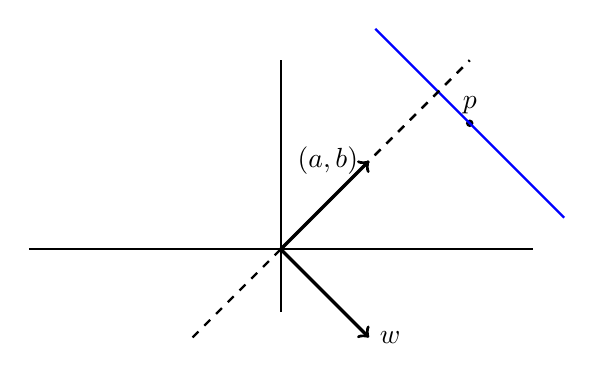
\begin{tikzpicture}[scale=0.8]
		\def\vx{3}
		\def\vy{2}
		\def\wx{4}
		\def\wy{1}	
		\def\tv{3.0}
		\def\tw{1.4}
		\def\taa{1.5}
		\def\tab{-1.5}
		\def\rr{\tv*\vy-\tv*\wy}	
		\def\ss{\tv*\wx-\tv*\vx}		
		\def\rrm{-\tw*\vy+\tw*\wy}	
		\def\ssm{-\tw*\wx+\tw*\vx}		
		\draw[thick,-] (-4,0) -- (4,0);
		\draw[thick,-] (0,-1) -- (0,3);
		%\node[inner sep=1.5pt,fill,circle] at (\vx,\vy) {};
		\draw[fill] (\vx,\vy) circle [radius=0.05];
		\node[above] at (\vx,\vy) {$p$};
		% 		\draw[very thick,->] (0,0) -- (\vx,\vy) node[above]{$v_0$};
		% 		\draw[very thick,->] (0,0) -- (\wx,\wy) node[above]{\;$v$};
		\draw[very thick,->] (0,0) -- (\tw*\wx-\tw*\vx,-\tw*\vy+\tw*\wy) node[right]{$w$};
		\draw[thick,blue,-] (\vx- \tab*\vx + \tab*\wx ,\vy - \tab*\vy + \tab*\wy) --  (\vx- \taa*\vx + \taa*\wx ,\vy - \taa*\vy + \taa*\wy);
		\draw[very thick,->] (0,0) -- (\tw*\vy-\tw*\wy,\tw*\wx-\tw*\vx) node[left]{$(a,b)$};
		\draw[dashed, thick,-] (0,0) -- (\rr,\ss);
		\draw[dashed, thick,-] (0,0) -- (\rr,\ss);
		\draw[dashed, thick,-] (\rrm,\ssm) -- (0,0);
		%\draw[dashed,thick] (0,0) (\tw*\wx,\tw*\wy) -- (\vx+\tw*\wx,\vy+\tw*\wy+0.1);
		%\node[inner sep=1.5pt,fill,circle,blue] at (\vx+\tw*\wx+0.04*\wx,\vy+\tw*\wy+0.04*\wy)  {};
		%\node[right] at (\vx+\tw*\wx,\vy+\tw*\wy+0.1){$v+tw$};
		\end{tikzpicture}
	\end{center} 
	
	En  este caso  es sencillo buscar un vector ortogonal. $w = (b,-a)$.
\end{frame}



\begin{frame}	
	Observemos que por la ley del paralelogramo si $p$ en la recta, entonces $p + t (-b,a)$ también está en la recta. 
	
	\vskip .4cm
	
Ver en GeoGebra: \href{https://www.geogebra.org/m/twzzezb3}{\beamergotobutton{https://www.geogebra.org/m/twzzezb3}}
		
	\vskip .4cm
		
	\begin{proposicion}
		Sean $(a,b),(x_0,y_0)\in\R^2$ con $(a,b)\neq0$.  La recta perpendicular a $(a,b)$ que pasa por $(x_0,y_0)$ es
		\begin{align*}
		L=\left\{(x_0,y_0)+t(b,-a)\mid t\in\R\right\} 
		\end{align*}
		
	\end{proposicion}
	
\end{frame}



\begin{frame}
	\begin{ejemplo}
		Encontrar una representación paramétrica para la recta que contiene los puntos $(2,2)$ y y es perpendicular a $(2,1)$.
	\end{ejemplo}	
	\begin{solucion} \pause
		\vskip .4cm
		
		El vector ortogonal a $(2,1)$  es $(1,-2)$. Luego:
		
		\begin{align*}
		L&=\left\{(2,2)+t(1,-2)\mid t\in\R\right\} \\
		&= \left\{(2 +t,2-2t)\mid t\in\R\right\}
		\end{align*}
		\qed
	\end{solucion}
\end{frame}



\begin{frame}{Recta entre dos puntos}
	
	Bien es sabido que s\'olo hay una recta que pasa por dos puntos dados $p,q\in\R^2$. Graficamente esta es:
	\begin{center}
		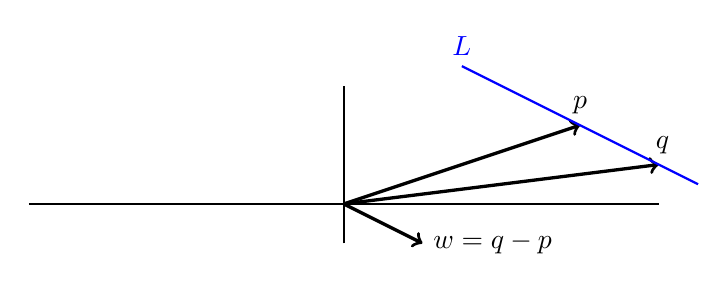
\begin{tikzpicture}[yscale=0.5]
		\def\vx{3}
		\def\vy{2}
		\def\wx{4}
		\def\wy{1}	
		\def\tv{3.0}
		\def\tw{1.4}
		\def\taa{1.5}
		\def\tab{-1.5}
		\def\rr{\tv*\vy-\tv*\wy}	
		\def\ss{\tv*\wx-\tv*\vx}		
		\def\rrm{-\tw*\vy+\tw*\wy}	
		\def\ssm{-\tw*\wx+\tw*\vx}		
		\draw[thick,-] (-4,0) -- (4,0);
		\draw[thick,-] (0,-1) -- (0,3);
		%\node[inner sep=1.5pt,fill,circle] at (\vx,\vy) {};
		\draw[very thick,->] (0,0) -- (\vx,\vy) node[above]{$p$};
		\draw[very thick,->] (0,0) -- (\wx,\wy) node[above]{\;$q$};
		\draw[very thick,->] (0,0) -- (\wx-\vx,\wy-\vy) node[right]{$w=q-p$};
		\draw[thick,blue,-] (\vx- \tab*\vx + \tab*\wx ,\vy - \tab*\vy + \tab*\wy) node[above] {$L$} --  (\vx- \taa*\vx + \taa*\wx ,\vy - \taa*\vy + \taa*\wy);
		% 		\draw[very thick,->] (0,0) -- (\tw*\vy-\tw*\wy,\tw*\wx-\tw*\vx) node[left]{$(a,b)$};
		% 		\draw[dashed, thick,-] (0,0) -- (\rr,\ss);
		% 		\draw[dashed, thick,-] (0,0) -- (\rr,\ss);
		% 		\draw[dashed, thick,-] (\rrm,\ssm) -- (0,0);
		%\draw[dashed,thick] (0,0) (\tw*\wx,\tw*\wy) -- (\vx+\tw*\wx,\vy+\tw*\wy+0.1);
		%\node[inner sep=1.5pt,fill,circle,blue] at (\vx+\tw*\wx+0.04*\wx,\vy+\tw*\wy+0.04*\wy)  {};
		%\node[right] at (\vx+\tw*\wx,\vy+\tw*\wy+0.1){$v+tw$};
		\end{tikzpicture}
	\end{center} 
	La manera m\'as f\'acil de describir dicha recta es usando la forma param\'etrica. 
	
	\
	
	En efecto, del gr\'afico vemos que $L$ es la recta que pasa por $p$ con direcci\'on $w=p-q$.
	
\end{frame}

\begin{frame}
	
	Lo anterior se resume en lo siguiente:
	
	
	\vskip .4cm
	
	
	\begin{block}{Afirmaci\'on}
		Sean $p,q\in\R^2$ y $w=p-q$. Entonces la \'unica recta que pasa por ambos puntos es
		\begin{align*}
		L = \{p + tw: t \in \R\}. 
		\end{align*}
		
	\end{block}
	
	
\end{frame}


\begin{frame}{Segmento entre dos puntos}
	La representación paramétrica también es útil para describir el conjunto de los puntos que se encuentran en el segmento de línea entre dos puntos dados. 
	
	\
	
	M\'as precisamente, el segmento entre $p$ y $q$ consiste en todos los puntos de la forma
	\begin{equation*}
	p + t(q-p)\quad  \text{con}\quad 0 \le t \le 1.
	\end{equation*}
	
	Como $t$ ``va'' de 0 a 1,  podemos pesar que recorremos el segemento desde
	\begin{itemize}
		\item	$p$, esto es cuando $t=0$, a
		\item $q$, esto es cuando $t=1$. 
	\end{itemize}
	
	
\end{frame}


\begin{frame}\frametitle{Planos en $\R^3$}
		Comenzaremos, con la ecuación normal del plano
		
		\vskip .3cm 
	\begin{figure}[h]
		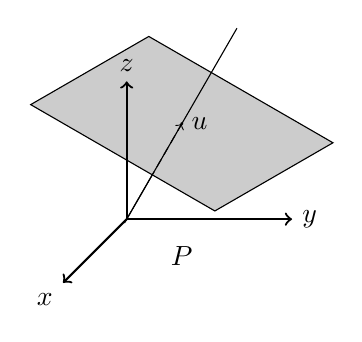
\begin{tikzpicture}[plane/.style={trapezium,draw,fill=black!20,trapezium left angle=60,trapezium right angle=120,minimum height=1.5cm},scale=0.7]
		\node (p)[plane,rotate=-30] at (2*0.5,2*0.866,0){.};
		\draw[rotate=-30] (p.center) edge ++(0,2cm) edge[densely dashed] (p.south) (p.south) edge ++(0,-1cm);
		\draw[->] (0,0,0) -- (2*0.5,2*0.866,0) node[right]{$u$};
		\draw[thick,->] (0,0,0) -- (3,0,0) node[right]{$y$};
		\draw[thick,->] (0,0,0) -- (0,2.5,0) node[above]{$z$};
		\draw[thick,->] (0,0,0) -- (0,0,3) node[anchor=north east]{$x$};
		\node [right] at (1.2,-0.1,1.5) {$P$};
		\end{tikzpicture}
		\caption{El plano $P$ y $u$, un vector  perpendicular al plano.}
	\end{figure} 
	

\end{frame}




\begin{frame}\frametitle{Planos en $\R^3$. Definición implícita}
		
	\begin{definicion} Sean $a,b, c,d \in \R$ tal que $(a,b,c) \ne (0,0,0)$ y sea 
		\begin{equation*}
		P = \{(x,y,z): ax +by +cz =d\}.
		\end{equation*}
		Entonces diremos que $P$  es  un \textit{plano con ecuación implícita}\index{plano en $\R^3$!ecuación implícita}  $ax +by +cz =d$ y  que $(a,b,c)$ es un \textit{vector normal al plano $P$.}
	\end{definicion} 
\vskip .4cm\pause
	 A esta forma de describir el plano también suele llamársela la \textit{ecuación normal del plano.}
	\vskip .4cm\pause

	Observar que la ecuación $ ax +by +cz =d$ no es más que la ecuación $\la(x,y,z),(a,b,c) \ra=d$. 	
	\vskip 1.2cm
\end{frame}



\begin{frame}
	\begin{ejemplo}
		El plano determinado por la ecuación
		\begin{equation*}
		2x - y 	+ 3z = 	5
		\end{equation*}
		es perpendicular al vector $(2, - 1, 3)$. 
		\vskip .4cm\pause
		¿Puntos del plano? Fijamos dos coordenadas y despejamos la tercera.
		\vskip .4cm\pause
		Por  ejemplo,  sea $x = 1$, $y = 1$ y despejamos $z$:
		\begin{equation*}
		3z 	= 5 - 2 + 1 = 4,
		\end{equation*}
		luego $z = \displaystyle\frac43$ y entonces
		\begin{equation*}
		(1,1,\frac43)
		\end{equation*}
		es un punto en el plano.
	\end{ejemplo}
\end{frame}



\begin{frame}
	Se dice que dos planos son \textit{paralelos} (en el 3-espacio) si sus vectores normales son paralelos,  es decir son proporcionales. 
	
	\vskip .8cm\pause
	
	Se dice que son \textit{perpendiculares} si sus vectores normales son perpendiculares. 
	
	\vskip .8cm\pause
	
	El \textit{ángulo entre dos planos} se define como el ángulo entre sus vectores normales.
	
	\vskip .4cm
	\vskip 2cm
	
\end{frame}



\begin{frame}\frametitle{Ecuación paramétrica del plano en $\R^3$}
  	
		\begin{definicion}
		Sean $v, w_1,w_2 \in \R^3$ tal que  $w_1$,$w_2$ no  nulos y tal que $w_2$ no sea un múltiplo de $w_1$. Sea 
		\begin{equation*}
		P = \{v + sw_1 + tw_2: s,t \in \R\}. 
		\end{equation*}
		Diremos entonces que  \textit{$P$ es el  plano a través de $v$ paralelo a los vectores $w_1$ y $w_2$.}\index{plano en $\R^3$!ecuación paramétrica} 
	\end{definicion}
\vskip .4cm
	


\end{frame}

\begin{frame}
	Si 
	\begin{equation*}
	P = \{v + sw_1 + tw_2: s,t \in \R\},
	\end{equation*}
	entonces el vector $v$ pertenece al plano y el plano 
	\begin{equation*}
	P_0 = \{sw_1 + tw_2: s,t \in \R\}
	\end{equation*}
	es el plano que pasa por el origen y paralelo a $P$. 
\end{frame}

\begin{frame}
	
	Si $P = \{(x,y,z): ax +by +cz =d\}$ con $a\ne 0$.
	\vskip .4cm
	Podemos poner $x$ en función de  $y$, $z$ y los datos. Así obtenemos una ecuación paramétrica de $P$. 
	
	\begin{equation*}
		 ax +by +cz =d \qquad \Rightarrow\qquad x = -\frac{b}{a} y-\frac{c}{a} z +d
	\end{equation*}
	
	Luego
	\begin{align*}
	P &= \{( -\frac{b}{a} y-\frac{c}{a} z +d, y, z): y, z \in \R \}\\	
	&= \{(d,0,0)+ y( -\frac{b}{a} , 1, 0) + z( -\frac{c}{a} , 0, 1): y, z \in \R \}.
	\end{align*}
	
	
	\vskip .4cm\pause
	Se puede hacer de forma análoga cuando $b\ne 0$ o $c \ne 0$. 
	
		\vskip .4cm\pause

\end{frame}

\begin{frame}
		\begin{ejemplo}
		Sea $P = \{(x,y,z): x -2y +z =1\}$. 
		\vskip .4cm
		Como  $x -2y +z =1$ sii  $x = 2y-z +1$, tenemos que
		\begin{equation*}
		P = \{(2y-z +1,y,z): y,z \in \R\},
		\end{equation*}\pause
		o,  escrito de una forma más estándar,
		\begin{equation*}
		P = \{(2s-t +1,s,t): s,t \in \R\}. 
		\end{equation*}
		
		También podemos escribir
		\begin{equation*}
		P = \{(1,0,0) + s(2,1,0) + t(-1,0,1): s,t \in \R\}. 
		\end{equation*}
		\qed
		
	\end{ejemplo}
\end{frame}





\begin{frame}
	¿Cómo obtenemos la ecuación normal del plano?
	\vskip .4cm\vskip .4cm\pause
	Si encontramos $u \ne 0$ tal que $\la u,w_1 \ra =0$ y $\la u,w_2 \ra =0$, entonces $ \la  sw_1 + tw_2, u \ra =0$ para  $s,t$ arbitrarios y 
	\begin{equation*}
	P_0 = \{(x,y,z): \la (x,y,z),u \ra =0\}. 
	\end{equation*}\pause	\vskip .1cm
	Sea $d = \la v, u \ra$, entonces $\la v + sw_1 + tw_2, u\ra = \la v , u\ra =d$, para $s,t$ arbitrarios. Es decir
	\begin{equation*}
	P = \{(x,y,z): \la (x,y,z),u \ra =d\}. 
	\end{equation*}
\end{frame}



\begin{frame}
		\begin{ejemplo}
		Sea $P = \{ (1,1,0) + s(-1,0,-1) + t(0,1,-2): s,t \in \R\}$. Encontrar la ecuación implicita de $P$.
		\end{ejemplo}
		\begin{solucion}\pause
			Sea $u= (a,b,c)$,  entonces 
			\begin{align*}
			\la u,(-1,0,-1) \ra = 0 \quad &\Leftrightarrow \quad -a -c=0 \quad\Leftrightarrow   \quad a = -c, \\
			\la u,(0,1,-2) \ra = 0 \quad &\Leftrightarrow \quad b -2c=0 \quad\,\Leftrightarrow \quad b=2c.
			\end{align*} 
			Luego $u=(-c,2c,c)$. Si, por ejemplo, $c=1$, $\Rightarrow$ $u=(-1,2,1)$, luego:
			\begin{equation*}
			P_0 = \{(x,y,z): -x+2y+z =0\}. 
			\end{equation*}
			Como $\la (1,1,0),(-1,2,1) \ra = 1 $, obtenemos
			\begin{align*}
			P &= \{(x,y,z): \la (x,y,z),(-1,2,1) \ra =1\} \\
			&= \{(x,y,z): -x+2y+z =1\}.
			\end{align*}
			\qed
		\end{solucion}
		

\end{frame}





\end{document}

